% !TEX encoding = UTF-8 Unicode
% !TEX spellcheck = en_US

\documentclass[conference,letterpaper]{IEEEtran}
% If the IEEEtran.cls has not been installed into the LaTeX system files,
% manually specify the path to it:
% \documentclass[conference]{../sty/IEEEtran}
\IEEEoverridecommandlockouts
\overrideIEEEmargins



%\documentclass[conference]{IEEEtran}
% If the IEEEtran.cls has not been installed into the LaTeX system files, 
% manually specify the path to it:
% \documentclass[conference]{../sty/IEEEtran} 


% some very useful LaTeX packages include:

\usepackage{cite}      % Written by Donald Arseneau
\usepackage{graphicx}  % Written by David Carlisle and 
\usepackage{psfrag}    % Written by Craig Barratt, Michael C. Grant,
\usepackage{color}
\usepackage{subfigure} % Written by Steven Douglas Cochran
\usepackage{url}       % Written by Donald Arseneau
\usepackage{stfloats}  % Written by Sigitas Tolusis
\usepackage{amsmath}   % From the American Mathematical Society
\usepackage{bm}        % Für fettgedruckte Formelzeichen
%Use:
\interdisplaylinepenalty=2500
\usepackage{array}
\usepackage{epsfig}

\usepackage{calc}
\usepackage{amssymb}
\usepackage{amstext}

\usepackage{multicol}
\usepackage{pslatex}
%\usepackage{apalike}
\usepackage[ngerman]{babel}

\usepackage{siunitx}
\usepackage{algpseudocode}
\usepackage{algorithm}

\graphicspath{{Chapters/Experimental_Results/Experimental_Validation/}}

%\usepackage{caption}
%\usepackage{subcaption}

% correct bad hyphenation here
\hyphenation{op-tical net-works semi-conduc-tor IEEEtran}

% Für Deutsche Umlaute
\usepackage[utf8]{inputenc}

\begin{document}

% paper title
%\title{Optimal Modelling for in Process Identification of Robot Models}
\title{Sensitivity-based Model Reduction for In-Process Identification of Industrial Robots Inverse Dynamics}

% author names and affiliations
% use a multiple column layout for up to three different
% affiliations
\author{\authorblockN{Björn Volkmann, Daniel Kaczor, Mathias Tantau, Moritz Schappler and Tobias Ortmaier}
\authorblockA{\textit{Institute of Mechatronic Systems, Leibniz University Hanover, Germany}\\
Email: \{bjoern.volkmann, mathias.tantau\}@imes.uni-hannover.de}}

% make the title area
\maketitle

\begin{abstract}
This paper presents a sensitivity-based approach for optimal model design and identification of the dynamics of a state-of-the-art industrial robot considering process-related restrictions.
The possibility of parameter excitation for subsequent identification of the model parameters is severely limited due to restrictions imposed by the process environment, especially the limited available workspace. 
Without sufficient parameter excitation, a satisfactory quality of the full model identification cannot be achieved, since non-excited parameters cannot be identified correctly.  
Furthermore, optimal excitation requires time-consuming calculations and distinct experiments during which the robot is not available for daily operation. 
It is therefore of interest to use process-related trajectories instead of dedicated excitation trajectories, which is expected to deteriorate the identifiability of the model parameters.
For this reason, the presented method uses a sensitivity-based approach allowing model order reduction in the identification process. The resulting model contains only those parameters excited by the excitation trajectory. For process-related trajectories this implies the model being limited to parameters relevant for the process. 
In experiments with a standard serial-link industrial robot controlled by standard industrial programmable logic control and servo inverters it is shown that the method produces significantly reduced models with a good measure of identifiability and quality.
\end{abstract}

% keywords
\begin{keywords}
Model order reduction; Sensitivity; Identification; Industrial Robot
\end{keywords}

% Will be ignored for other modes.
%\IEEEpeerreviewmaketitle

% !TEX encoding = UTF-8 Unicode
% !TEX spellcheck = en_US
\section{Introduction}
\label{subsec:Introduction}

Highly dynamic handling processes such as pick and place applications are common in industrial robotics.
One of the most important quality factors, besides the lowest possible cycle time, is the accuracy of the performed movements. The more dynamic a motion sequence is supposed to be, the more demanding it is to achieve the accuracy requirements. For this reason, there are many approaches in the field of robotics aiming to improve the accuracy of the system under the influence of highly dynamic movements. 

One of the most widespread methods to achieve this goal is the model-based feedforward control of the motor torque for a given motion profile.
This method is based on the complete knowledge of the dynamics model and its parameters. 
In most cases, however, this knowledge is not completely available. 
For this reason the missing model parameters have to be identified with a suitable excitation. 
A widely used method to perform this excitation is the parameter excitation with Fourier-based trajectories \cite{Park.2006,Swevers.1997}.
The coefficients of the Fourier series are optimized for minimal sensitivity of the identification to measurement disturbances. 
\cite{Goutier.2012} and \cite{Goutier.2014} present a method in which the identification of the parameters of industrial robots is carried out with the aid of an additional payload with exactly known mass. 
It is attached to the end-effector to improve the identifiability and excitation of the parameters during the identification process.
The separate identification of individual model parameters is presented in \cite{Wernholt.2006}. 
Here, a three-step sequential routine for the isolated identification of the friction and dynamics parameters and the values for elasticities of an industrial robot is performed. By the individual identification using different exitation trajectories for each parameter an improvement of the identifiability of the respective parameters can be achieved.
Further, \cite{Khalil.2007} presents a procedure for individual identification of the additional payload at the end-effector of the robot.

These approaches for the dynamics identification of a robot mostly use industrial hardware, but they do not take into account the process-related restrictions that apply when dealing with a robot that is already integrated into the production process. 
In the process environment, a robot is mostly surrounded by other systems such as conveyor belts or other robots so that it can only move in a part of its actually possible workspace. This fact strongly limits the possibility to perform a sufficient and generally valid trajectory for a successful parameter excitation or makes it impossible in many cases. As a result, the model parameters cannot be identified with sufficient accuracy and the methods mentioned above can only be used to a very limited extent. 
Furthermore, an interruption of the running process and additional working hours are necessary to perform a dedicated excitation trajectory. 
% This is not desired in most cases, since additional working hours are necessary for the trajectory generation. 
A separate sequential identification with different excitation trajectories or the use of an additional testing payload is also not applicable in the process.

To address these limitations, we present a sensitivity-based method that allows to identify the model parameters and/or reduce the robot model during the robot's designated process. In this way the model adapts to the circumstances of the given excitation. It is not necessary to optimize and run an additional excitation trajectory and the process does not have to be stopped at any time and can be continued unaffectedly. 
The presented method is demonstrated by identifying necessary parameters of the inverse dynamics model under process conditions of the 6-degrees-of-freedom (dof) standard serial industrial robot \textsc{Cloos QRC 350}. 
The main contributions of this paper are:
\begin{itemize}
    \item identification of the dynamics parameters of an industrial robot under on-site conditions with a
    \item scheme for reduction of parameter complexity based on given workspace and trajectories
    \item using only standard industrial hardware.
\end{itemize}

The remainder of this paper is organized as follows: Sec.\,\ref{sec:TheoreticalBackground} gives a short view on the used inverse dynamics model and its minimal parameter formulation. Furthermore, the theoretical principles of parameter identification are presented. Sec.\,\ref{sec:Experiments} describes the performed experiments. 
The experiment design is introduced and the investigated processes are presented. 
Beside the consideration of the signal processing, the developed algorithm is introduced in detail.
Sec.\,\ref{sec:Experimental_Results} provides experimental results, demonstrating the effectiveness of the proposed method. Sec.\,\ref{sec:Conclusion} concludes the paper.

% !TEX encoding = UTF-8 Unicode
% !TEX spellcheck = en_US
% !TEX root = ../../ICMA2020.tex

\section{Theoretical Background}
\label{sec:TheoreticalBackground}



%% Included Chapters
% !TEX encoding = UTF-8 Unicode
% !TEX spellcheck = en_US
% !TEX root = ../../../ICMA2020.tex

\subsection{Dynamics Model of Serial Robots}
This subsection describes the dynamics model of the 6-axis robot.
The joint torques $\boldsymbol{\tau}$ of all axes required for the feedforward control can be calculated by
%
\begin{equation}
\label{eq:model_equation1}
\begin{split}
\boldsymbol{\tau}=
\boldsymbol{M}(\boldsymbol{q}) \ddot{\boldsymbol{q}}+\boldsymbol{c}(\boldsymbol{q}, \dot{\boldsymbol{q}})+\boldsymbol{g}(\boldsymbol{q})+\boldsymbol{h}(\dot{\boldsymbol{q}}).
\end{split}
\end{equation}
%
Herein $\boldsymbol{q}$, $\dot{\boldsymbol{q}}$ and $\ddot{\boldsymbol{q}}$ represent the joint angles, velocities and accelerations given by the motion planning. $\boldsymbol{M}$ denotes the mass matrix, $\boldsymbol{c}$ the Coriolis effects and $\boldsymbol{g}$ the gravitational effects.
The friction model is represented by $\boldsymbol{h}$ with
%
\begin{equation}
h_{j}=f_{\mathrm{c}, j} \operatorname{sgn}\left(\dot{{q}}_{j}\right)+f_{\mathrm{v}, j} \dot{q}_{j},
\end{equation}
%
where $f_{\mathrm{c}, j}$ represents the Coulomb friction coefficient for joint $j$ and $f_{\mathrm{v}, j}$ the viscous friction coefficient.
The gear transmission between motor and link side is omitted for the sake of simplifying the equations. Measured motor velocities and estimated motor torques are transformed accordingly.

By expressing the rigid body dynamics with the inertial parameters (drive train inertia, mass, first and second moment of mass) and by using a linear friction model, (\ref{eq:model_equation1}) can be expressed in a linear form \cite{Khalil.2006}.
%
This regressor form
%
\begin{equation}
\boldsymbol{\tau}
=
\boldsymbol{X}'(\boldsymbol{q}, \dot{\boldsymbol{q}},\ddot{\boldsymbol{q}}) \boldsymbol{\theta}'
=
\boldsymbol{X}(\boldsymbol{q}, \dot{\boldsymbol{q}},\ddot{\boldsymbol{q}}) \boldsymbol{\theta}
\label{eq:model_regressor}
\end{equation}
%
with regression matrix $\boldsymbol{X}$ and parameter vector $\boldsymbol{\theta}$
can be given with a full set of parameters (on the left hand side, noted with a dash) or in a parameter minimal form (right hand side).
Only the latter form of the parameters can be identified within one identification cycle.
The general model $\boldsymbol{X}'$/$\boldsymbol{\theta}'$ uses 66 parameters for the rigid body dynamics.
For each of the six joints two additional parameters represent the Coulomb and viscous friction.

The right hand side of (\ref{eq:model_regressor}) expresses the minimal parametric model with 23 base inertial parameters.
The chosen parameter vector $\boldsymbol{\theta}$ to be identified therefore contains 35 entries and is shown in appendix \ref{sec:MinparamVector}.
%
Since some of the robot links possess symmetries, assumptions about their center of mass and products of inertia were made.
Further, a differential gear couples joints 5 and 6, similar to the robot example in \cite{M.Gautier.1995}.
This prevents the use of the direct determination of the base inertial parameters with the geometric approach from \cite{Khalil.2006}.
Instead, a purely symbolic approach is chosen: the relation $\boldsymbol{\theta}=\boldsymbol{K} \boldsymbol{\theta}'$ leads to a linear system of equations $\boldsymbol{X}' = \boldsymbol{X}'\boldsymbol{K}$.
It is solved symbolically for the unknown $\boldsymbol{K}$ with the computer algebra system \textsc{Maple}, leading to the base parameter formulation $\boldsymbol{X}$/$\boldsymbol{\theta}$.
For the implementation the regressor matrix of the energy instead of the dynamics is used, following \cite{M.Gautier.1995, Khalil.2006}.
% !TEX encoding = UTF-8 Unicode
% !TEX spellcheck = en_US
% !TEX root = ../../../ICMA2020.tex

\subsection{Parameter Estimation}
\label{subsec:ParameterEstimation}


For parameter identification the model equations from \eqref{eq:model_equation1} are transformed into the parameter linear matrix notation

\begin{equation} \label{eq:ParameterEstimation_regressor}
    \boldsymbol{\tau} = \boldsymbol{X}(\boldsymbol{q}, \dot{\boldsymbol{q}},\ddot{\boldsymbol{q}}) \boldsymbol{\theta},
\end{equation}

where $\boldsymbol{\tau}$ is the joint torque vector, $\boldsymbol{X}$ denotes the regression matrix and $\boldsymbol{\theta} \in \mathbb{R}^{35}$ is the parameter vector. Using a sufficient number of samples in the estimation process leads to an over-determined system of linear equations:

\begin{equation} \label{eq:ParameterEstimation_problem}
\begin{aligned}
    \boldsymbol{y} &= \boldsymbol{C} \boldsymbol{\theta} + \boldsymbol{\epsilon}, \\
    \begin{pmatrix}
        \boldsymbol{\tau}(t_1) \\
        \vdots \\
        \boldsymbol{\tau}(t_N) \\
    \end{pmatrix} &= 
    \begin{pmatrix}
        \boldsymbol{X}(t_1) \\
        \vdots \\
        \boldsymbol{X}(t_N) \\
    \end{pmatrix} \boldsymbol{\theta} +
    \begin{pmatrix}
        \boldsymbol{e}(t_1) \\
        \vdots \\
        \boldsymbol{e}(t_N) \\
    \end{pmatrix}.
\end{aligned}
\end{equation}

Here $\boldsymbol{y}$ contains the $N$ samples of the torque vector $\boldsymbol{\tau}$, $\boldsymbol{C}$ denotes the design matrix and $\boldsymbol{\epsilon}$ is the vector of errors.

Equation \eqref{eq:ParameterEstimation_problem} can be solved for $\boldsymbol{\theta}$ using a least squares estimator. The weighted least squares (WLS)  \cite{Gautier.2013,M.Gautier.1995,V.Bargsten.2013,Swevers.1997} is used to account for different levels of noise in the measurements: 
\begin{equation} \label{eq:ParameterEstimation_WLS}
    \begin{aligned}
	    \hat{\boldsymbol{\theta}} &= \arg \min_{{\boldsymbol{\theta}}} (\boldsymbol{y} - \boldsymbol{C} \boldsymbol{\theta})^\mathrm{T} \boldsymbol{W} (\boldsymbol{y} - \boldsymbol{C} \boldsymbol{\theta}) \\
	    &= (\boldsymbol{C}^\mathrm{T} \boldsymbol{W} \boldsymbol{C})^{-1} \boldsymbol{C}^\mathrm{T} \boldsymbol{W} \boldsymbol{y}.
	\end{aligned}
\end{equation}
Matrix $\boldsymbol{W}$ contains the weights of the individual samples, see also Sec.\,\ref{subsec:SignalProcessing}.


% !TEX encoding = UTF-8 Unicode
% !TEX spellcheck = en_US
% !TEX root = ../../../ICMA2020.tex

\subsection{Optimal Excitation}
\label{subsec:OptimalExcitation_Result}


In consideration of the optimized trajectories from Sec.\,\ref{subsec:ExperimentScenario} the robot parameters are estimated using the WLS method according to \eqref{eq:ParameterEstimation_WLS}. The filtering of the respective measurement data in the frequency domain yields nearly noise free estimates of the joint angular positions, velocities and accelerations. According to \cite{Khalil.2006} it is possible to estimate the relative standard deviation $\sigma_{i}^*$ of the identified parameters for the LS method under the assumption of a deterministic design matrix and the error $\boldsymbol{e}$ as zero-mean additive independent Gaussian noise. Applying this to the WLS method with $\mathrm{var}(\boldsymbol{y}) = \boldsymbol{W}^{-1}$ yields the covariance matrix

\begin{equation}\label{eq:ParaVar}
	\begin{aligned}
&	\mathrm{var}(\hat{\boldsymbol{\theta}}) &= {}& \mathrm{var}((\boldsymbol{C}^\mathrm{T} \boldsymbol{W} \boldsymbol{C})^{-1} \boldsymbol{C}^\mathrm{T} \boldsymbol{W} \boldsymbol{y}) \\
&								&= {}& (\boldsymbol{C}^\mathrm{T} \boldsymbol{W} \boldsymbol{C})^{-1} \boldsymbol{C}^\mathrm{T} \boldsymbol{W} \mathrm{var}(\boldsymbol{y}) \boldsymbol{W}^\mathrm{T} \boldsymbol{C} (\boldsymbol{C}^\mathrm{T} \boldsymbol{W} \boldsymbol{C})^{-\mathrm{T}} \\
&								&= {}& (\boldsymbol{C}^\mathrm{T} \boldsymbol{W} \boldsymbol{C})^{-1},
	\end{aligned}
\end{equation}

and the relative standard deviation of the identified parameters

\begin{equation}\label{eq:ParaVar_rel}
	\sigma_{i}^* = \frac{\sigma_{i}}{\left| \hat{\theta}_i \right|} \text{ with } \sigma_{i}^2 = \mathrm{var}(\hat{\boldsymbol{\theta}})_{ii}.
\end{equation}

%The $i$-th diagonal element $\sigma_{i}^2$ of $\mathrm{var}(\hat{\boldsymbol{\theta}})$ corresponds to the standard deviation $\sigma_i$ of parameter $i$. 
The estimated parameters and standard deviations for trajectories \textit{A} and \textit{B} are given in Tab.\,\ref{tab:ParamTheta}. For convenience the derived models will now be called model A and B respectively. It can be seen that parameters with a relatively high standard deviation have small identified values compared to other parameters with a lower standard deviation. These parameters could either not be sufficiently excited or their contribution to the model is negligible \cite{Khalil.2006}.

\begin{table}
	\caption{Estimated parameters for model A and B.}\label{tab:ParamTheta}
	\centering
	\begin{tabular}[h]{|r||c|c||c|c|}\hline
		% !TEX encoding = UTF-8 Unicode
% !TEX spellcheck = en_US
		& \multicolumn{2}{c||}{Model A}		& \multicolumn{2}{c|}{Model B}		\\ \hline 
    $i$ & $\hat{\theta}_{i}$   & $\sigma_{i}^*$ (\%)&	$\hat{\theta}_{i}$   & $\sigma_{i}^*$ (\%) \\ \hline 
    1     & 19.763 & 0.522 & 16.174 & 0.802 \\ %\hline 
    2     & 23.798 & 0.678 & 28.312 & 0.491 \\ %\hline 
    3     & -0.850 & 6.927 & -1.076 & 4.028 \\ %\hline 
    4     & 17.162 & 0.532 & 12.657 & 0.587 \\ %\hline 
    5     & 37.957 & 0.054 & 38.748 & 0.054 \\ %\hline 
    6     & 11.684 & 1.003 & 10.435 & 1.145 \\ %\hline 
    7     & 0.768 & 3.551 & 0.973 & 3.581 \\ %\hline 
    8     & 1.785 & 3.275 & 2.284 & 2.991 \\ %\hline 
    9     & 8.666 & 0.450 & 9.451 & 0.429 \\ %\hline 
    10    & 0.266 & 12.323 & -1.272 & 3.196 \\ %\hline 
    11    & 5.913 & 0.189 & 5.537 & 0.244 \\ %\hline 
    12    & 12.163 & 0.072 & 12.203 & 0.051 \\ %\hline 
    13    & 4.249 & 1.242 & 5.555 & 0.394 \\ %\hline 
    14    & 0.108 & 4.814 & 0.027 & 30.466 \\ %\hline 
    15    & 0.162 & 2.088 & -0.002 & 162.640 \\ %\hline 
    16    & -0.058 & 5.650 & 0.122 & 2.802 \\ %\hline 
    17    & 0.200 & 0.563 & 0.224 & 0.495 \\ %\hline 
    18    & 0.225 & 0.647 & 0.280 & 0.559 \\ %\hline 
    19    & 1.254 & 0.048 & 1.265 & 0.042 \\ %\hline 
    20    & 0.074 & 2.560 & 0.065 & 2.664 \\ %\hline 
    21    & 0.043 & 1.407 & 0.027 & 1.881 \\ %\hline 
    22    & 0.037 & 0.737 & 0.036 & 0.794 \\ %\hline 
    23    & 0.135 & 0.241 & 0.137 & 0.308 \\ %\hline 
    24    & 76.809 & 0.281 & 75.944 & 0.195 \\ %\hline 
    25    & 117.258 & 0.154 & 104.977 & 0.148 \\ %\hline 
    26    & 47.677 & 0.190 & 43.214 & 0.180 \\ %\hline 
    27    & 4.125 & 0.174 & 3.292 & 0.215 \\ %\hline 
    28    & 1.454 & 0.428 & 1.245 & 0.362 \\ %\hline 
    29    & 0.834 & 0.379 & 0.753 & 0.301 \\ %\hline 
    30    & 62.856 & 0.468 & 65.058 & 0.364 \\ %\hline 
    31    & 36.423 & 0.560 & 45.561 & 0.403 \\ %\hline 
    32    & 17.903 & 0.553 & 16.107 & 0.411 \\ %\hline 
    33    & 1.039 & 0.346 & 1.314 & 0.283 \\ %\hline 
    34    & 0.434 & 1.365 & 0.647 & 0.702 \\ %\hline 
    35    & 0.426 & 0.256 & 0.538 & 0.208 \\

		\hline
	\end{tabular}
\end{table}

The absolute and relative model errors $e_{j}$ and $e^*_{j}$ for models A and B according to \eqref{eq:absError} and \eqref{eq:relError} are given in Tab.\,\ref{tab:errorModelA} and Tab.\,\ref{tab:errorModelB} respectively. Greater deviations between the model predictions and the measured torques result from the noise on the measured torques and the dynamic behavior of the controlled system like the characteristics of the controller and the compensation of overshoots. It can be seen that both models produce approximately the same model prediction error for all trajectories. This leads to the conclusion that the model parameters were sufficiently excited during the experiments and both models can be used as reference for the process-based parameter estimation.

\begin{table}
	\caption{Prediction error for model A.}\label{tab:errorModelA}
	\centering
	\begin{tabular}[h]{|r||c|c||c|c|}\hline
		joint & \multicolumn{2}{c||}{Trajectory A} & \multicolumn{2}{c|}{Trajectory C} \\ \hline	 
$j$     & $e_j$ (Nm) & $e_j^*$ (\%)& $e_j$ (Nm) & $e_j^* (\%)$ \\ \hline	 
1	 & 23.298	 & 15.172	 & 16.974	 & 15.218	 \\	 
2	 & 44.518	 & 12.507	 & 49.945	 & 13.734	 \\	 
3	 & 16.607	 & 12.699	 & 18.592	 & 17.442	 \\	 
4	 & 1.083	 & 12.732	 & 1.149	 & 16.312	 \\	 
5	 & 1.202	 & 15.857	 & 1.082	 & 14.261	 \\	 
6	 & 0.282	 & 11.850	 & 0.286	 & 12.521	 \\	 

		\hline
	\end{tabular}
\end{table}

\begin{table}
	\caption{Prediction error for model B.}\label{tab:errorModelB}
	\centering
	\begin{tabular}[h]{|r||c|c||c|c|}\hline
		joint & \multicolumn{2}{c||}{Trajectory B} & \multicolumn{2}{c|}{Trajectory C} \\ \hline	 
$j$     & $e_j$ (Nm) & $e_j^*$ (\%)& $e_j$ (Nm) & $e_j^* (\%)$ \\ \hline	 
1	 & 21.439	 & 15.081	 & 16.846	 & 15.104	 \\	 
2	 & 48.997	 & 16.175	 & 50.935	 & 14.007	 \\	 
3	 & 18.451	 & 16.852	 & 17.985	 & 16.873	 \\	 
4	 & 1.182	 & 19.174	 & 1.209	 & 17.169	 \\	 
5	 & 0.964	 & 12.734	 & 1.069	 & 14.088	 \\	 
6	 & 0.208	 & 12.561	 & 0.404	 & 17.733	 \\	 

		\hline
	\end{tabular}
\end{table}
% !TEX encoding = UTF-8 Unicode
% !TEX spellcheck = en_US
% !TEX root = ../../ICMA2020.tex

\section{Experiments}
\label{sec:Experiments}


%% Included Chapters
% !TEX encoding = UTF-8 Unicode
% !TEX spellcheck = en_US
\subsection{Robot Testbed}
\label{subsec:RobotTestbed}
For experimental evaluations and demonstration of the potential the presented approach was testet on the state-of-the-art serial industrial  robot \textsc{Cloos QRC 350} designed for highly dynamic and precise processes such as assembly or welding tasks. 
The robot is controlled by a standard industrial PLC and servo inverters from the company \textsc{Lenze}. 
For data processing and calculation of the implemented algorithm a standard desktop computer with \textsc{Matlab} software was used. 
However, in the perspective all calculations can also be carried out directly on the PLC. 
The test setup for the experiments and the validation is shown in Fig.\,\ref{fig:testbench}. 
% For a better understanding, the definition of the kinematic parameters $l_1$ -- $l_6$ of the robot are added to this figure.

\begin{figure}[!ht]             % Einbetten in figure wie gehabt
    \centering                  % zentrierte Ausrichtung, optional
    \def\svgwidth{\textwidth/2}    
        % die Bildbreite muss auf diese Weise festgelegt werden!
    %\input{Chapters/Experiments/Robot_Testbed/CLOOS_cover.pdf_tex}  
    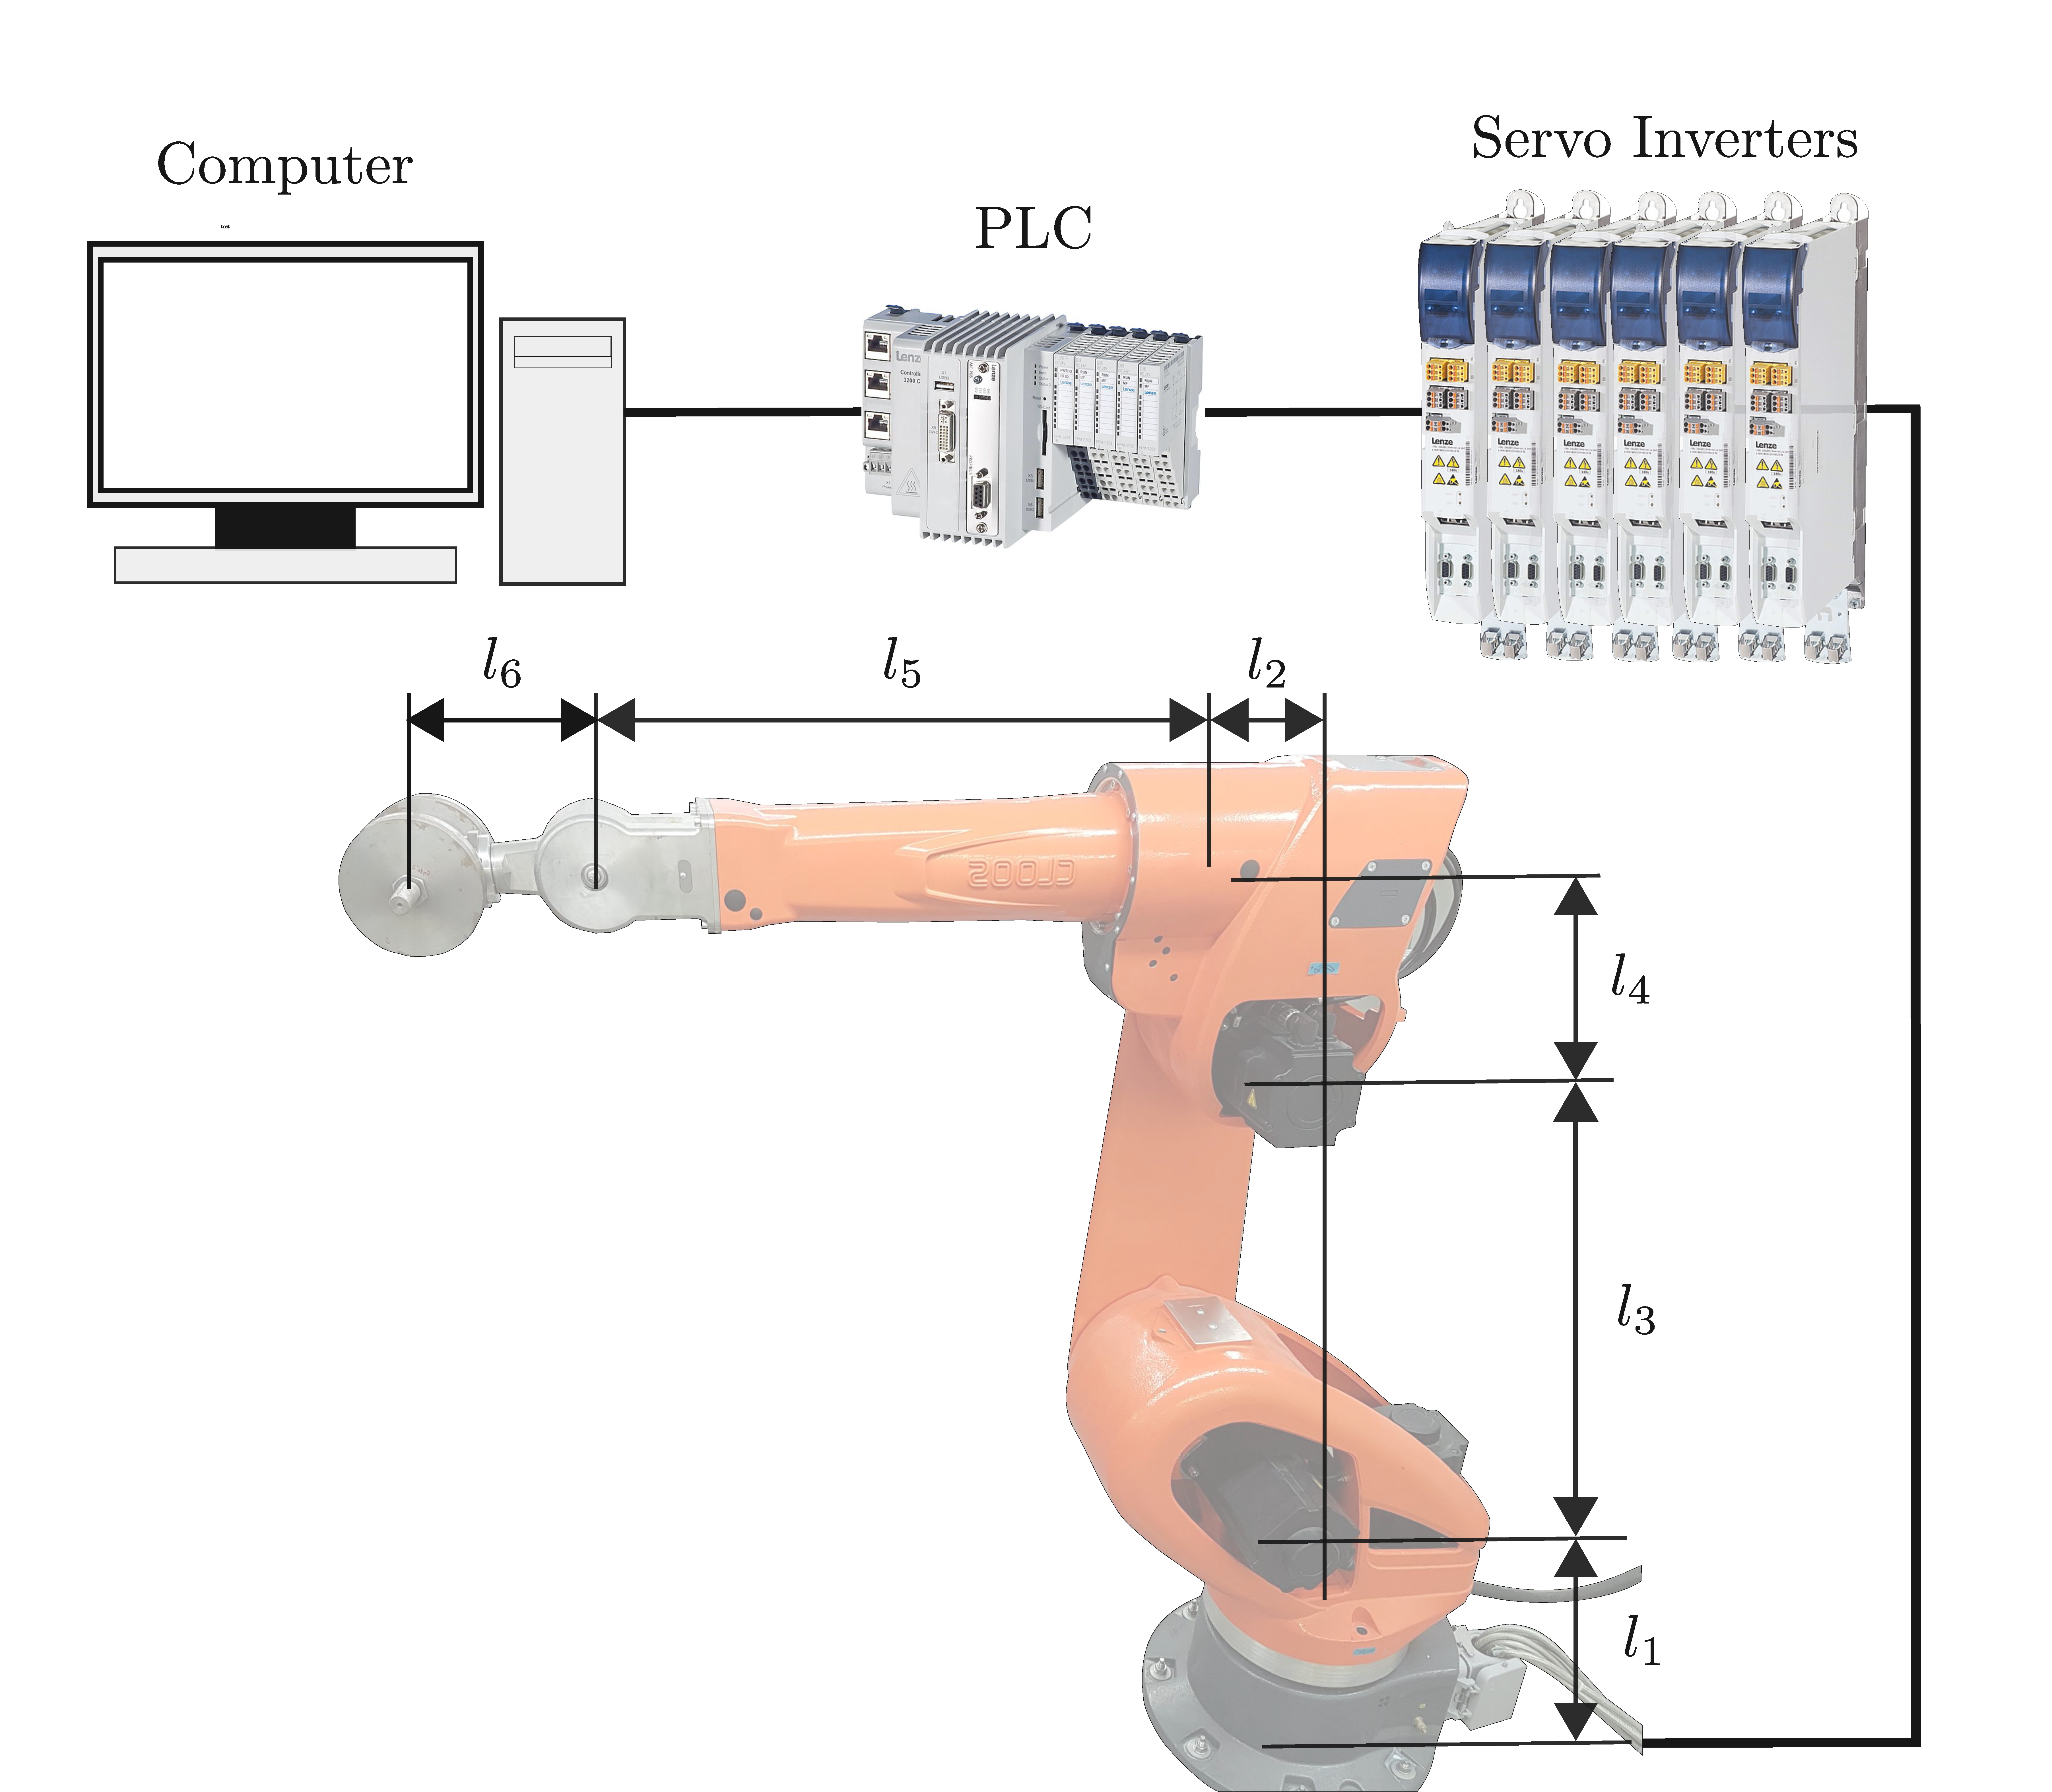
\includegraphics[width=8.6cm]{Chapters/Experiments/Robot_Testbed/Cloos_cover} 
               \caption{Experiment setup with a 6-dof \textsc{Cloos QRC 350} industrial robot, PLC and servo inverters and a desktop computer for development.}
   \label{fig:testbench}
\end{figure}


% pdf Größe reduzieren mit dem Windows Befehl
%gswin64 -dNOPAUSE -dBATCH -sDEVICE=pdfwrite -dCompatibilityLevel=1.4 -dPDFSETTINGS=/prepress -sOutputFile=prev_events_impressions_small.pdf prev_events_impressions.pdf

% Auflösung: 
%-dPDFSETTINGS=/screen   (screen-view-only quality, 72 dpi images)
%-dPDFSETTINGS=/ebook    (low quality, 150 dpi images)
%-dPDFSETTINGS=/printer  (high quality, 300 dpi images)
%-dPDFSETTINGS=/prepress (high quality, color preserving, 300 dpi imgs)
%-dPDFSETTINGS=/default  (almost identical to /screen)

% Weitere Informationen: http://milan.kupcevic.net/ghostscript-ps-pdf/
% !TEX encoding = UTF-8 Unicode
% !TEX spellcheck = en_US

\subsection{Experiment Scenario}
\label{subsec:ExperimentScenario}

As described in Sec.\,\ref{subsec:Introduction}, a parameter identification in the process environment is rarely feasible without restrictions regarding the available workspace. For this reason, the approach of the method presented in this paper is based on performing the necessary parameter identification directly in the running process. To illustrate this situation, the proposed method is applied to two different tasks widely used in industry. These processes are presented in more detail in the following paragraph. 
\begin{itemize}
\item Process 1: The robot performs a highly dynamic \textit{pick and place} motion between two pre-defined areas in the workspace (see Fig.\,\ref{fig:Process1}.a). To create a set of \textit{pick-and-place} cycles the points on both areas are generated randomly.
\item Process 2: The end-effector of the robot has to trace the edges of a horizontal square (see Fig.\,\ref{fig:Process1}.b).
\end{itemize}
To validate the identified parameters, different trajectories of the same type are used for each process. For process 1 a new set of points is randomly generated using a uniform distribution. For process 2 the trajectory is given an offset in the $x$-$y$-plane.

%\begin{figure*}[tb]
%  \vspace{-0.2cm}
%  \centering
%   \includegraphics[width = 18cm]{Chapters/Experiments/Experimental_Design/SzenarienKompakt.pdf}
%  \caption{Representation of process 1 and 2 and the restricted robot workspace.}
%  \label{fig:Process1}
%  \vspace{-0.1cm}
%\end{figure*}

%\begin{figure}[tb]
%  \vspace{-0.2cm}
%  \centering
%   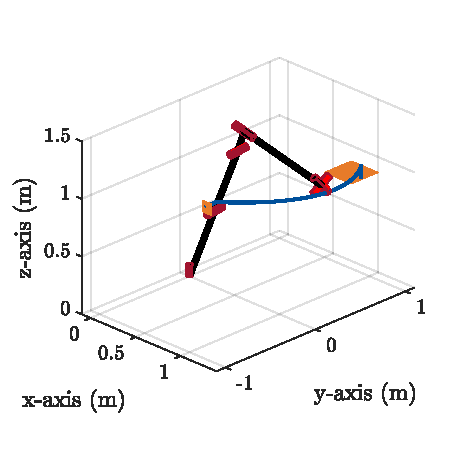
\includegraphics[width = 7.5cm]{Chapters/Experiments/Experimental_Design/Szenario_PnP.pdf}
%  \caption{Representation of process 1 in the robot workspace.}
%  \label{fig:Process1}
%  \vspace{-0.1cm}
%\end{figure}

%\begin{figure}[tb]
%  \vspace{-0.2cm}
%  \centering
%   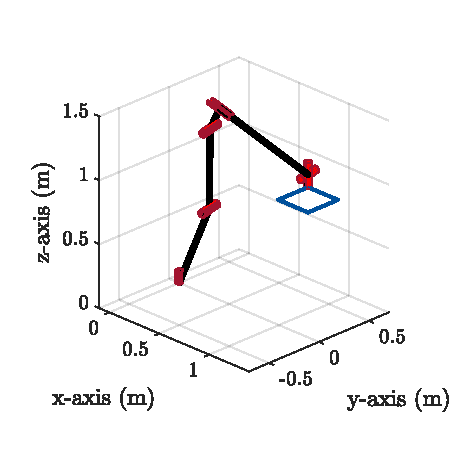
\includegraphics[width = 7.5cm]{Chapters/Experiments/Experimental_Design/Szenario_Square.pdf}
%  \caption{Representation of process 2 in the robot workspace.}
%  \label{fig:Process2}
%  \vspace{-0.1cm}
%\end{figure}

To evaluate the results of the process-based parameter identification a classical parameter identification with three different optimized excitation trajectories is also carried out. The first excitation trajectory uses the full workspace of the robot to get the best possible identification results. For the second trajectory the available robot workspace is restrained to simulate the identification process under practical conditions in the industrial environment. A representation of the used workspace is given in Fig.\,\ref{fig:Process1}.c. The complete half-sphere represents the full workspace. The marked area denotes the restrained workspace. The optimized excitation trajectories are generated according to Sec.\,\ref{subsec:OptimalExcitation}. The trajectory which uses the full workspace has a condition number of 6.76 and will be called \textit{trajectory A}. The trajectory in the restrained workspace has a condition number of 7.71 and will be called \textit{trajectory B}. Restraining the available workspace generally leads to higher condition numbers of the generated excitation trajectory. The third trajectory is used to validate both models derived from the optimal excitation and will be called \textit{trajectory C}. Like \textit{trajectory A}, \textit{trajectory C} is generated in the full workspace of the robot but uses a different set of \textsc{Fourier}-coefficients, due to the heuristic nature of the genetic algorithm. The identification was performed without model-based feedforward control.

%\begin{figure}[tb]
%  \vspace{-0.2cm}
%  \centering
%   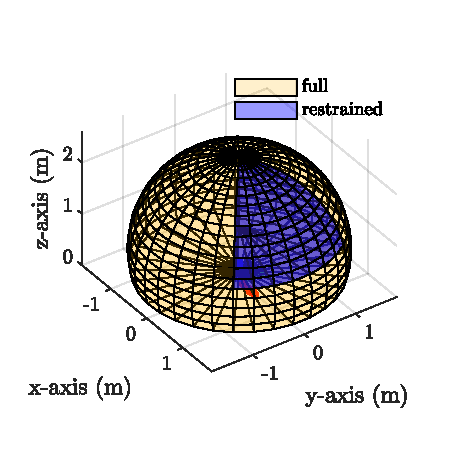
\includegraphics[width = 7.5cm]{Chapters/Experiments/Experimental_Design/TaskSpace.pdf}
%  \caption{Representation of the used workspace during optimized excitation.}
%  \label{fig:TaskSpace}
%  \vspace{-0.1cm}
%\end{figure}


%\begin{figure*}[tb]
%   \centering
%   \begin{subfigure}{0.3\textwidth}
%        %\vspace{-0.2cm}
%        \centering
%            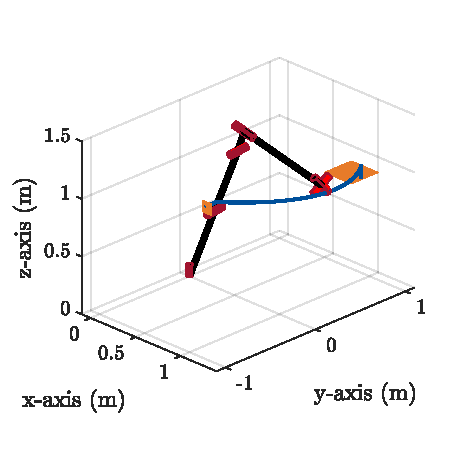
\includegraphics[width = \textwidth]{Chapters/Experiments/Experimental_Design/Szenario_PnP.pdf}
%        \caption{Representation of process 1 in the robot workspace.}
%        \label{fig:Process1}
%        %\vspace{-0.1cm}
%    \end{subfigure}%
%    
%    \begin{subfigure}{0.3\textwidth}
%        %\vspace{-0.2cm}
%        \centering
%            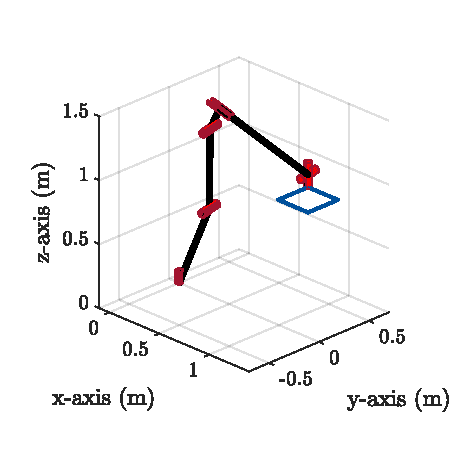
\includegraphics[width = \textwidth]{Chapters/Experiments/Experimental_Design/Szenario_Square.pdf}
%        \caption{Representation of process 2 in the robot workspace.}
%        \label{fig:Process2}
%        %\vspace{-0.1cm}
%    \end{subfigure}%
%    
%    \begin{subfigure}{0.3\textwidth}
%        %\vspace{-0.2cm}
%        \centering
%            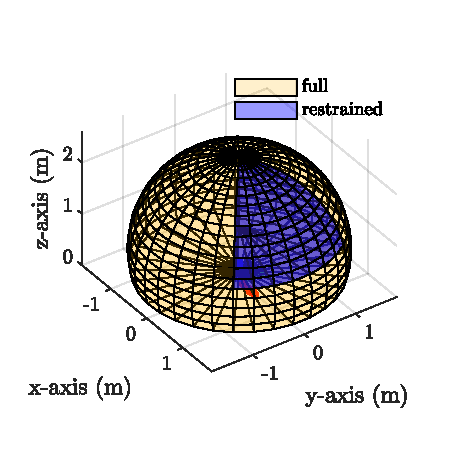
\includegraphics[width = \textwidth]{Chapters/Experiments/Experimental_Design/TaskSpace.pdf}
%        \caption{Representation of the used workspace during optimized excitation.}
%       \label{fig:TaskSpace}
%        %\vspace{-0.1cm}
%    \end{subfigure}%
%    \caption{Representation of process 1 and 2 and the restricted robot workspace.}
%\end{figure*}

\begin{figure*}[tb]
  \vspace{-0.2cm}
  \centering
    %\subfigure[Representation of process 1 in the robot workspace.]{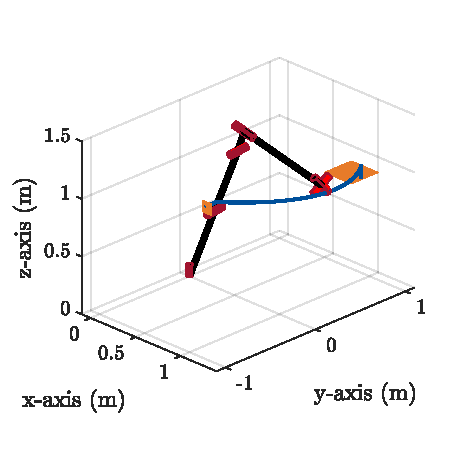
\includegraphics[width = 5.5cm]{Chapters/Experiments/Experimental_Design/Szenario_PnP.pdf}}
    %\subfigure[Representation of process 2 in the robot workspace.]{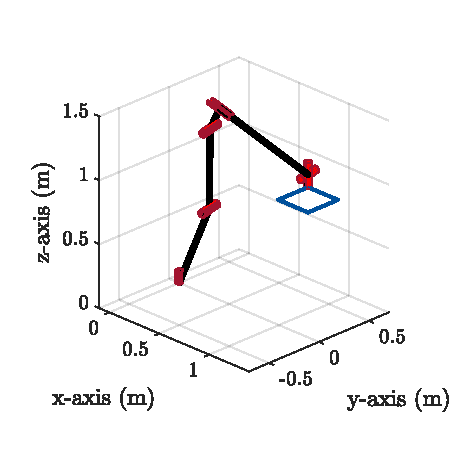
\includegraphics[width = 5.5cm]{Chapters/Experiments/Experimental_Design/Szenario_Square.pdf}}
    %\subfigure[Representation of the used workspace during optimized excitation.]{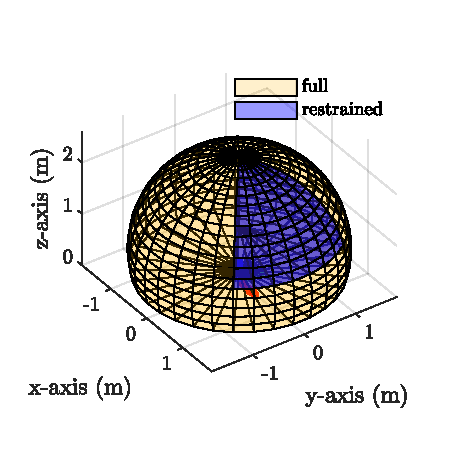
\includegraphics[width = 5.5cm]{Chapters/Experiments/Experimental_Design/TaskSpace.pdf}}
    \includegraphics{Chapters/Experiments/Experiment_Scenario/SzenarienKompakt.pdf}
  \vspace{-0.2cm}
  \caption{Representation of process 1 and 2 and the workspace used for optimization.}
  \label{fig:Process1}
  \vspace{-0.3cm}
\end{figure*}
% !TEX encoding = UTF-8 Unicode
% !TEX spellcheck = en_US
\subsection{Signal Processing}
\label{subsec:SignalProcessing}
All experiments described in Sec.\,\ref{subsec:ExperimentScenario} are carried out multiple times with the same set of parameters. Over $N_\text{r}=50$ repetitions of each experiment the mean of the joint angular positions $\overline{\boldsymbol{q}}(t_p)$ and the measured torques $\overline{\boldsymbol{\tau}}(t_p)$ are calculated for every time step $t_p$. 

In the case of the \textsc{Fourier} series the frequency spectrum of the excitation is known, which allows for additional filtering of the position measurements: 
The discrete \textsc{Fourier} transform of the mean position measurements $\overline{\boldsymbol{q}}$ is calculated and only the first $n_\mathrm{h}+1$ \textsc{Fourier} coefficients are retained. These correspond to the offset, the base frequency and the $n_\mathrm{h}-1$ harmonics. Utilizing this filter technique yields nearly noise-free estimates of the joint angular positions.
A possible loss of information is tolerated in favor of reduced noise.
The same filter technique is used in \cite{Olsen.2002} and \cite{Stueckelmaier.}. 
Because of the averaging of the measurement data and the additional filtering for the \textsc{Fourier} series the derivatives for the joint angular velocities and accelerations can be calculated numerically for all experiments.

%Since periodic \textsc{Fourier} series are used as excitation trajectories, no leakage errors are introduced due to the allowed settling time of the system. 

To take into account the different signal-to-noise ratios in each joint, the WLS method is used for parameter estimation. The measurement points are weighted using the inverse of the covariance matrix of the measured torque. The noise of the torque measurements in all joints $j$ in every time step $t_p$ can be estimated using the equation for the sample variance
\begin{equation}\label{eq:var_tau}
	\sigma^2_{j,p} = \frac{1}{N_\textit{r}-1} \sum\limits_{k=1}^{N_\textit{r}} (\tau_{k,j} (t_p) - \overline{\tau}_j(t_p))^2,
\end{equation}
where (k) refers to the repetitions of the experiment.
The matrix $\boldsymbol{W}$ is then defined as:
\begin{equation}\label{eq:WLS_Gew}
	\boldsymbol{W} = \mathrm{diag}(\boldsymbol{W}_1^{-1}, \boldsymbol{W}_2^{-1}, \hdots, \boldsymbol{W}_6^{-1})
\end{equation}
	with
\begin{equation}
	\boldsymbol{W}_j = \mathrm{diag}(\sigma^2_{j,1}, \sigma^2_{j,2}, \hdots, \sigma^2_{j,p}).
\end{equation}
Since the measurements are assumed to be independent, $\boldsymbol{W}$ is a diagonal matrix.
All measurements used for this evaluation were taken when the robot was at rest and in the controlled state.


% !TEX encoding = UTF-8 Unicode
% !TEX spellcheck = en_US
% !TEX root = ../../../ICMA2020.tex

\subsection{Model Reduction Algorithm}
A parameter identification in a process not optimized for this purpose leads to a significantly worse identifiability compared to an optimized excitation trajectory due to the sub-optimal excitation of the individual parameters.
In order to still perform a parameter estimation directly on a process the robot model has to be reduced.
According to \cite{Brun2001} two factors can be distinguished that lead to poor identifiability and a high condition number: sensitivity problems and collinearity problems. 
Sensitivity can differ between parameters so that some parameters affect the output only negligibly while others dominate. Collinearity means that the effect of one parameter is compensated by the interplay of other parameters.

Many model order reduction techniques strive to establish a new basis without multi-collinearities, which is possibly even orthogonal. 
Here these approaches are prohibited by the fact that the interpretability of the base parameters should be preserved in the sense of the linear combination of physical parameters in (\ref{eq:Parametersatz}). 
A different approach is to delete parameters that are involved in collinearity problems \cite{Akinniyi2017}, but this could change the prediction of the model considerably if the respective parameter is important. Therefore, only the sensitivity problem is addressed here.
As the model can be written linear in the parameters, see \eqref{eq:model_regressor}, it is possible to remove those parameters with a low sensitivity on a per-parameter basis.
The parameter sensitivities depend on the excitation but not on the parameter values. For a particular excitation the sensitivity matrix is given by the design matrix $\boldsymbol{C}$. To characterize the sensitivity of a parameter $i$ with a single value the mean of the respective column $\overline{c}_i$ of $\boldsymbol{C}$ over all joints is used:
%\begin{equation}\label{eq:mean_Sensitivity}
%	\overline{c}_i = \frac{1}{6N} \sum_{i = 1}^{6N} \left| \boldsymbol{c}_i \right| \text{ with } \boldsymbol{C} = (\boldsymbol{c}_1, \boldsymbol{c}_2, %\hdots, \boldsymbol{c}_i).
%\end{equation}
\begin{equation}\label{eq:mean_Sensitivity}
	\overline{c}_i = \frac{1}{6N} \| \boldsymbol{c}_i \|_1 \text{ with } \boldsymbol{C} = (\boldsymbol{c}_1, \boldsymbol{c}_2, \hdots, \boldsymbol{c}_i).
\end{equation}

The model error that is introduced by removing a particular parameter is evaluated using the error between the measured data $\boldsymbol{\tau}$ and the model prediction $\hat{\boldsymbol{\tau}}$. The mean absolute error 
\begin{equation}\label{eq:absError}
	e_{k,j} = \frac{1}{N}  \sum\limits_{p=1}^{N} \left| \tau_j(t_p) - \hat{\tau}_{k,j}(t_p) \right|,
\end{equation}
and the relative error
\begin{equation}\label{eq:relError}
	e^*_{k,j} = \frac{e_{k,j}}{\frac{1}{N} \sum\limits_{p=1}^{N} \left| \tau_j(t_p) \right|}
\end{equation}
are calculated in every step $k$ for all joints $j$. If removing a parameter would lead to a large model error, this parameter is retained.

The following is a detailed description of the proposed approach, explained along the pseudo code in algorithm\,\ref{alg:ModelReductionAlgorithm}. It can be characterized as a \textit{backward stepwise selection} \cite{Volinsky1997} because starting from the full model parameters are removed successively.

The algorithm begins with calculating the initial design matrix $\boldsymbol{C}_0$ for the full model (line 1). It is checked if the design matrix is of full rank, so that all parameters are identifiable. Given that the parameter estimation is to be performed directly on a process and not with an optimized trajectory, some parameters may not be identifiable. In such a case the parameters in question must be removed prior to the model reduction.

If the design matrix is of full rank, a first parameter estimation with the full model needs to be carried out (line 2). Based on that the absolute and relative model errors $e_{0,j}$ and $e^*_{0,j}$ are calculated (line 3). These values will be the reference to determine if a parameter is negligible for the model.

\begin{algorithm}[ht]
\caption{Pseudo code of the model reduction algorithm.}\label{alg:ModelReductionAlgorithm}
	\begin{algorithmic}[1]
	%\State Load data
	%\State Calculate design matrix $\boldsymbol{C}$
	\State Examine rank of design matrix $\boldsymbol{C}_k$ (initially $\boldsymbol{C}_0$)
	\State Calculate $\hat{\boldsymbol{\theta}}_{0}$ using WLS
	\State Calculate $e_{0,j}$, $e^*_{0,j}$
	\State Initialize $I$ and $E$
	\For {$k =1,2,\ldots,n_i$}
		%\State Construct design matrix with parameters $i \in I$
		%\State Calculate $\overline{c}_i$ for $i \in I$
		\State Calculate $\arg \min_{i} (\overline{c}_i)$ with $i \in I \wedge i \notin E$
		\State Remove parameter $i$
		\State Calculate $\hat{\boldsymbol{\theta}}_{k}$ using WLS
		\State Calculate $e_{k,j}$, $e^*_{k,j}$
		\If {$\frac{e^*_{k,j}}{e^*_{0,j}} \geq e_{\text{tol}} \text{ } \forall j$}
			\State Add parameter $i$ to $E$
		\Else
			\State Remove parameter $i$ from $I$
		\EndIf
	\EndFor
	\end{algorithmic}
\end{algorithm}

Sets $I$ (included) and $E$ (essential) are initialized  (line 4): Set $I$ represents the parameters which are still included in the model in a given iteration and is initialized to contain all parameters. Set $E$ contains all parameters which are indispensable for the model. The friction may be indispensable for the model if all joints perform a sufficient motion during the observed process. In this case  $E$ will include the friction parameters, otherwise set $E$ is initialized empty.

The model reduction is then performed in a loop which iterates over all $n_i=35$ parameters in the model. First the design matrix needs to be constructed with the parameters defined by $I$ and $E$ (line 6). Then the parameter with the lowest sensitivity is determined using $\overline{c}_i$ from \eqref{eq:mean_Sensitivity} and removed from the model (line 7). With the resulting reduced model a parameter estimation is carried out using the WLS method and the absolute and relative model errors $e_{k,j}$ and $e^*_{k,j}$ are calculated (line 8 and 9).

In a final step it needs to be determined if the removed parameter is negligible for the model (line 10). The parameter can be considered negligible if the relative model error $e^*_{k,j}$ in step $k$ is within a pre-defined tolerance margin $e_{\mathrm{tol}}$ with respect to the reference value $e^*_{0,j}$ for all joints $j$.% Removing the friction parameters may result in a reduced model which is within the error tolerance, but the robustness of the parameter estimation is negatively impacted. This can be seen in a high condition number of the reduced model which means the parameters are not equally excited and therefore poorly identified. 

The advantage of the algorithm is that it removes unimportant parameters so that the model error keeps low, but since the condition number is not optimized directly its improvement may be small. Nevertheless, it has been found in several experiments that the condition number is also improved.
% !TEX encoding = UTF-8 Unicode
% !TEX spellcheck = en_US
\section{Experimental Results}
\label{sec:Experimental_Results}


%% Included Chapters
% !TEX encoding = UTF-8 Unicode
% !TEX spellcheck = en_US
% !TEX root = ../../../ICMA2020.tex

\subsection{Optimal Excitation}
\label{subsec:OptimalExcitation_Result}


In consideration of the optimized trajectories from Sec.\,\ref{subsec:ExperimentScenario} the robot parameters are estimated using the WLS method according to \eqref{eq:ParameterEstimation_WLS}. The filtering of the respective measurement data in the frequency domain yields nearly noise free estimates of the joint angular positions, velocities and accelerations. According to \cite{Khalil.2006} it is possible to estimate the relative standard deviation $\sigma_{i}^*$ of the identified parameters for the LS method under the assumption of a deterministic design matrix and the error $\boldsymbol{e}$ as zero-mean additive independent Gaussian noise. Applying this to the WLS method with $\mathrm{var}(\boldsymbol{y}) = \boldsymbol{W}^{-1}$ yields the covariance matrix

\begin{equation}\label{eq:ParaVar}
	\begin{aligned}
&	\mathrm{var}(\hat{\boldsymbol{\theta}}) &= {}& \mathrm{var}((\boldsymbol{C}^\mathrm{T} \boldsymbol{W} \boldsymbol{C})^{-1} \boldsymbol{C}^\mathrm{T} \boldsymbol{W} \boldsymbol{y}) \\
&								&= {}& (\boldsymbol{C}^\mathrm{T} \boldsymbol{W} \boldsymbol{C})^{-1} \boldsymbol{C}^\mathrm{T} \boldsymbol{W} \mathrm{var}(\boldsymbol{y}) \boldsymbol{W}^\mathrm{T} \boldsymbol{C} (\boldsymbol{C}^\mathrm{T} \boldsymbol{W} \boldsymbol{C})^{-\mathrm{T}} \\
&								&= {}& (\boldsymbol{C}^\mathrm{T} \boldsymbol{W} \boldsymbol{C})^{-1},
	\end{aligned}
\end{equation}

and the relative standard deviation of the identified parameters

\begin{equation}\label{eq:ParaVar_rel}
	\sigma_{i}^* = \frac{\sigma_{i}}{\left| \hat{\theta}_i \right|} \text{ with } \sigma_{i}^2 = \mathrm{var}(\hat{\boldsymbol{\theta}})_{ii}.
\end{equation}

%The $i$-th diagonal element $\sigma_{i}^2$ of $\mathrm{var}(\hat{\boldsymbol{\theta}})$ corresponds to the standard deviation $\sigma_i$ of parameter $i$. 
The estimated parameters and standard deviations for trajectories \textit{A} and \textit{B} are given in Tab.\,\ref{tab:ParamTheta}. For convenience the derived models will now be called model A and B respectively. It can be seen that parameters with a relatively high standard deviation have small identified values compared to other parameters with a lower standard deviation. These parameters could either not be sufficiently excited or their contribution to the model is negligible \cite{Khalil.2006}.

\begin{table}
	\caption{Estimated parameters for model A and B.}\label{tab:ParamTheta}
	\centering
	\begin{tabular}[h]{|r||c|c||c|c|}\hline
		% !TEX encoding = UTF-8 Unicode
% !TEX spellcheck = en_US
		& \multicolumn{2}{c||}{Model A}		& \multicolumn{2}{c|}{Model B}		\\ \hline 
    $i$ & $\hat{\theta}_{i}$   & $\sigma_{i}^*$ (\%)&	$\hat{\theta}_{i}$   & $\sigma_{i}^*$ (\%) \\ \hline 
    1     & 19.763 & 0.522 & 16.174 & 0.802 \\ %\hline 
    2     & 23.798 & 0.678 & 28.312 & 0.491 \\ %\hline 
    3     & -0.850 & 6.927 & -1.076 & 4.028 \\ %\hline 
    4     & 17.162 & 0.532 & 12.657 & 0.587 \\ %\hline 
    5     & 37.957 & 0.054 & 38.748 & 0.054 \\ %\hline 
    6     & 11.684 & 1.003 & 10.435 & 1.145 \\ %\hline 
    7     & 0.768 & 3.551 & 0.973 & 3.581 \\ %\hline 
    8     & 1.785 & 3.275 & 2.284 & 2.991 \\ %\hline 
    9     & 8.666 & 0.450 & 9.451 & 0.429 \\ %\hline 
    10    & 0.266 & 12.323 & -1.272 & 3.196 \\ %\hline 
    11    & 5.913 & 0.189 & 5.537 & 0.244 \\ %\hline 
    12    & 12.163 & 0.072 & 12.203 & 0.051 \\ %\hline 
    13    & 4.249 & 1.242 & 5.555 & 0.394 \\ %\hline 
    14    & 0.108 & 4.814 & 0.027 & 30.466 \\ %\hline 
    15    & 0.162 & 2.088 & -0.002 & 162.640 \\ %\hline 
    16    & -0.058 & 5.650 & 0.122 & 2.802 \\ %\hline 
    17    & 0.200 & 0.563 & 0.224 & 0.495 \\ %\hline 
    18    & 0.225 & 0.647 & 0.280 & 0.559 \\ %\hline 
    19    & 1.254 & 0.048 & 1.265 & 0.042 \\ %\hline 
    20    & 0.074 & 2.560 & 0.065 & 2.664 \\ %\hline 
    21    & 0.043 & 1.407 & 0.027 & 1.881 \\ %\hline 
    22    & 0.037 & 0.737 & 0.036 & 0.794 \\ %\hline 
    23    & 0.135 & 0.241 & 0.137 & 0.308 \\ %\hline 
    24    & 76.809 & 0.281 & 75.944 & 0.195 \\ %\hline 
    25    & 117.258 & 0.154 & 104.977 & 0.148 \\ %\hline 
    26    & 47.677 & 0.190 & 43.214 & 0.180 \\ %\hline 
    27    & 4.125 & 0.174 & 3.292 & 0.215 \\ %\hline 
    28    & 1.454 & 0.428 & 1.245 & 0.362 \\ %\hline 
    29    & 0.834 & 0.379 & 0.753 & 0.301 \\ %\hline 
    30    & 62.856 & 0.468 & 65.058 & 0.364 \\ %\hline 
    31    & 36.423 & 0.560 & 45.561 & 0.403 \\ %\hline 
    32    & 17.903 & 0.553 & 16.107 & 0.411 \\ %\hline 
    33    & 1.039 & 0.346 & 1.314 & 0.283 \\ %\hline 
    34    & 0.434 & 1.365 & 0.647 & 0.702 \\ %\hline 
    35    & 0.426 & 0.256 & 0.538 & 0.208 \\

		\hline
	\end{tabular}
\end{table}

The absolute and relative model errors $e_{j}$ and $e^*_{j}$ for models A and B according to \eqref{eq:absError} and \eqref{eq:relError} are given in Tab.\,\ref{tab:errorModelA} and Tab.\,\ref{tab:errorModelB} respectively. Greater deviations between the model predictions and the measured torques result from the noise on the measured torques and the dynamic behavior of the controlled system like the characteristics of the controller and the compensation of overshoots. It can be seen that both models produce approximately the same model prediction error for all trajectories. This leads to the conclusion that the model parameters were sufficiently excited during the experiments and both models can be used as reference for the process-based parameter estimation.

\begin{table}
	\caption{Prediction error for model A.}\label{tab:errorModelA}
	\centering
	\begin{tabular}[h]{|r||c|c||c|c|}\hline
		joint & \multicolumn{2}{c||}{Trajectory A} & \multicolumn{2}{c|}{Trajectory C} \\ \hline	 
$j$     & $e_j$ (Nm) & $e_j^*$ (\%)& $e_j$ (Nm) & $e_j^* (\%)$ \\ \hline	 
1	 & 23.298	 & 15.172	 & 16.974	 & 15.218	 \\	 
2	 & 44.518	 & 12.507	 & 49.945	 & 13.734	 \\	 
3	 & 16.607	 & 12.699	 & 18.592	 & 17.442	 \\	 
4	 & 1.083	 & 12.732	 & 1.149	 & 16.312	 \\	 
5	 & 1.202	 & 15.857	 & 1.082	 & 14.261	 \\	 
6	 & 0.282	 & 11.850	 & 0.286	 & 12.521	 \\	 

		\hline
	\end{tabular}
\end{table}

\begin{table}
	\caption{Prediction error for model B.}\label{tab:errorModelB}
	\centering
	\begin{tabular}[h]{|r||c|c||c|c|}\hline
		joint & \multicolumn{2}{c||}{Trajectory B} & \multicolumn{2}{c|}{Trajectory C} \\ \hline	 
$j$     & $e_j$ (Nm) & $e_j^*$ (\%)& $e_j$ (Nm) & $e_j^* (\%)$ \\ \hline	 
1	 & 21.439	 & 15.081	 & 16.846	 & 15.104	 \\	 
2	 & 48.997	 & 16.175	 & 50.935	 & 14.007	 \\	 
3	 & 18.451	 & 16.852	 & 17.985	 & 16.873	 \\	 
4	 & 1.182	 & 19.174	 & 1.209	 & 17.169	 \\	 
5	 & 0.964	 & 12.734	 & 1.069	 & 14.088	 \\	 
6	 & 0.208	 & 12.561	 & 0.404	 & 17.733	 \\	 

		\hline
	\end{tabular}
\end{table}
% !TEX encoding = UTF-8 Unicode
% !TEX spellcheck = en_US
% !TEX root = ../../../ICMA2020.tex

\subsection{Process-Based Excitation}

One of the main advantages of the process-based approach is that both data collection and processing can be automated. Additionally, no special excitation trajectory has to be generated.
The parameter estimation is done as described in algorithm\,\ref{alg:ModelReductionAlgorithm} using the WLS method. The estimated parameters for process 1 and 2 are given in Tab.\,\ref{tab:ParamThetaProcess}. Here $\hat{\boldsymbol{\theta}}_{0}$ denotes the estimated parameters for the full model and $\hat{\boldsymbol{\theta}}_{\text{r}}$ denotes the estimated parameters for the reduced model. For both processes an error-tolerance $e_{\mathrm{tol}}$ of \SI{5}{\%} was chosen.

\begin{table}[tb]
	\caption{Estimated parameters for process 1 and 2.}\label{tab:ParamThetaProcess}
	\vspace{-0.2cm}
	\centering
	\begin{tabular}[h]{|r||c|c||c|c|}\hline
		% !TEX encoding = UTF-8 Unicode
% !TEX spellcheck = en_US
      & \multicolumn{2}{c||}{Process 1} & \multicolumn{2}{c|}{Process 2} \\ \hline
$i$     & $\hat{\theta}_{0,i}$ & $\hat{\theta}_{\text{r},i}$ & $\hat{\theta}_{0,i}$ & $\hat{\theta}_{\text{r},i}$ \\ \hline
1     & 9.952 & --    & -437.335 & 48.044 \\ %\hline
2     & 33.558 & 45.321 & 35.387 & -- \\ %\hline
3     & 1.541 & --    & 3.090 & -- \\ %\hline
4     & -13.419 & --    & 11.982 & -- \\ %\hline
5     & 43.786 & 43.928 & 40.110 & 43.342 \\ %\hline
6     & 2.154 & --    & 443.672 & -- \\ %\hline
7     & 1.686 & --    & -2.062 & -- \\ %\hline
8     & 5.073 & 1.163 & -106.802 & -- \\ %\hline
9     & -1.067 & --    & 2.602 & 14.090 \\ %\hline
10    & 6.866 & --    & -4.599 & -- \\ %\hline
11    & 3.132 & 3.446 & 6.693 & -- \\ %\hline
12    & 12.541 & 12.432 & 11.725 & 14.315 \\ %\hline
13    & 6.232 & --    & 7.899 & -- \\ %\hline
14    & -1.156 & --    & 1.804 & -- \\ %\hline
15    & 2.215 & --    & 3.139 & 2.998 \\ %\hline
16    & -2.247 & --    & -3.576 & -- \\ %\hline
17    & 0.233 & 0.336 & 0.259 & -- \\ %\hline
18    & 0.088 & --    & 0.189 & -- \\ %\hline
19    & 1.322 & 1.323 & 1.334 & 1.326 \\ %\hline
20    & 0.126 & --    & 0.093 & -- \\ %\hline
21    & -0.133 & --    & 0.097 & -- \\ %\hline
22    & 0.049 & 0.072 & 0.084 & 0.111 \\ %\hline
23    & 0.039 & --    & 0.040 & -- \\ %\hline
24    & 82.388 & 82.415 & 67.167 & 66.071 \\ %\hline
25    & 124.553 & 124.452 & 92.337 & 94.886 \\ %\hline
26    & 47.021 & 47.102 & 47.073 & 47.594 \\ %\hline
27    & 4.360 & 4.325 & 4.364 & -- \\ %\hline
28    & 1.151 & 1.150 & 0.849 & 0.945 \\ %\hline
29    & 0.664 & 0.665 & 0.718 & 0.719 \\ %\hline
30    & 73.001 & 72.674 & 128.156 & 132.694 \\ %\hline
31    & 90.762 & 87.536 & 84.485 & 79.244 \\ %\hline
32    & 45.309 & 45.794 & 27.302 & 26.225 \\ %\hline
33    & 2.007 & 1.973 & -4340.924 & -- \\ %\hline
34    & 1.072 & 1.140 & 3.247 & -- \\ %\hline
35    & 1.748 & 1.749 & 1.183 & 1.181 \\

		\hline
	\end{tabular}
\end{table}

For process 1 $15$ parameters were removed during the model reduction. The condition number of the full model for the excitation of process~1 is $61.7$. As a result of the model reduction, the condition number for the reduced design matrix was decreased to $8.46$. Because of the significantly lower condition number the parameter estimation becomes more robust. For process~1 the friction parameters can not be neglected since all joints perform a sufficient motion. During the model reduction of process~2 $16$ dynamics parameters and $3$ friction parameters were removed. A peculiarity of process~2 is that there is little to no movement in the joints 4 and 6. This results in a significantly higher condition number of $1632$ for the full model compared to process~1. This was reduced to $2.73$ during the model reduction. Since some joints perform little to no movement the respective friction parameters can be neglected and are removed by the model reduction algorithm. The model prediction errors for the process-models applied to the respective process are given in Tab.\,\ref{tab:errorProcessOnProcess}. Both models A and B yield similar model prediction errors for for process 1 and 2. Therefore only the model prediction errors for model A are displayed in Tab.\,\ref{tab:errorModelAOnProcess} to have a comparison to the model which was derived from the best possible excitation.% This is due to the fact that the models A and B are of similar quality when compared by their model errors as shown in section \ref{subsec:OptimalExcitation_Result}. The model prediction errors for model A and B on both processes are given in Tab. \ref{tab:errorModelAOnProcess} and \ref{tab:errorModelBOnProcess} respectively.

\begin{table}[tb]
	\caption{Prediction error for the process based models on their respective process.}\label{tab:errorProcessOnProcess}
	\vspace{-0.2cm}
	\centering
	\begin{tabular}[h]{|r||c|c||c|c|}\hline
		joint & \multicolumn{2}{c||}{Process 1} & \multicolumn{2}{c|}{Process 2} \\ \hline	 
$j$     & $e_j$ (Nm) & $e_j^*$ (\%)& $e_j$ (Nm) & $e_j^* (\%)$ \\ \hline	 
1	 & 21.563	 & 23.231	 & 17.937	 & 22.569	 \\	 
2	 & 25.332	 & 8.919	 & 30.617	 & 14.605	 \\	 
3	 & 9.423	 & 7.134	 & 15.359	 & 12.422	 \\	 
4	 & 2.037	 & 31.543	 & 0.892	 & 102.439	 \\	 
5	 & 0.384	 & 12.336	 & 0.464	 & 52.539	 \\	 
6	 & 0.239	 & 31.973	 & 0.213	 & 27.173	 \\	 

		\hline
	\end{tabular}
\end{table}

\begin{table}[tb]
	\caption{Prediction error for model A on process 1 and 2.}\label{tab:errorModelAOnProcess}
	\centering
	\vspace{-0.2cm}
	\begin{tabular}[h]{|r||c|c||c|c|}\hline
		joint & \multicolumn{2}{c||}{Process 1} & \multicolumn{2}{c|}{Process 2} \\ \hline	 
$j$     & $e_j$ (Nm) & $e_j^*$ (\%)& $e_j$ (Nm) & $e_j^* (\%)$ \\ \hline	 
1	 & 23.164	 & 24.955	 & 19.000	 & 23.908	 \\	 
2	 & 33.788	 & 11.897	 & 35.443	 & 16.907	 \\	 
3	 & 11.215	 & 8.490	 & 16.642	 & 13.459	 \\	 
4	 & 2.295	 & 35.531	 & 0.994	 & 114.172	 \\	 
5	 & 0.452	 & 14.522	 & 0.640	 & 72.497	 \\	 
6	 & 0.327	 & 43.626	 & 0.221	 & 28.249	 \\	 

		\hline
	\end{tabular}
\end{table}

%\begin{table}[tb]
%	\caption{Prediction error for model B on process 1 and 2.}\label{tab:errorModelBOnProcess}
%	\centering
%	\begin{tabular}[h]{|r||c|c||c|c|}\hline
%		joint & \multicolumn{2}{c||}{Process 1} & \multicolumn{2}{c|}{Process 2} \\ \hline	 
$j$     & $e_j$ (Nm) & $e_j^*$ (\%)& $e_j$ (Nm) & $e_j^* (\%)$ \\ \hline	 
1	 & 23.076	 & 24.861	 & 18.923	 & 23.810	 \\	 
2	 & 36.921	 & 13.000	 & 34.251	 & 16.338	 \\	 
3	 & 13.532	 & 10.244	 & 17.040	 & 13.781	 \\	 
4	 & 2.443	 & 37.824	 & 1.005	 & 115.508	 \\	 
5	 & 0.410	 & 13.157	 & 0.560	 & 63.379	 \\	 
6	 & 0.316	 & 42.275	 & 0.228	 & 29.097	 \\	 

%		\hline
%	\end{tabular}
%\end{table}

The removed model parameters are negligible for the observed process since without them the model error did not increase by more than \SI{5}{\%}. The parameters $5$, $12$, $19$ and $22$ had relatively low changes in their values throughout the model reduction and were estimated with similar values for all models. Removing them from the model also yields a significantly higher prediction error when compared to the other parameters.

It is only possible to evaluate the physical consistency (see e.g. \cite{Gautier.2013}) of the parameters 8, 10, 13, 15, 16, 20, 22 and 23 since not all of the model parameters are independently identifiable. The mentioned parameters are inertia values and therefore must be positive. For the reduced models of process 1 and 2 this is the case for all mentioned parameters which were kept in the model.

For the validation trajectories of both processes the design matrix was calculated using the desired values of the joint angular positions, accelerations and velocities. This was done because the models are expected to be used in a model-based feedforward control scheme which also uses the desired values. As already explained in Sec.\,\ref{subsec:OptimalExcitation_Result}, the greater deviations between the model predictions and the measured torques result from the noise on the measured torques and the dynamic behavior of the controlled system. This effect is the strongest in joints 4 and 5 for process~2 where nearly no motion is performed which results in a high signal-to-noise ratio.

It should be noted that the model reduction only keeps parameters which are needed to describe the joint torques of the observed process. Therefore the resulting models may not be generally applicable. The process based identification has to be repeated for every new process the robot has to perform, and the resulting model can only be applied to that process. The parameter estimation is done through the robot application, which has to be implemented on the controller regardless. Therefore no additional expenditure arises.

Despite the restraints applied on the workspace, the parameter estimation with an optimized trajectory could still be performed. However, restricting the robot workspace hampers the excitation of all parameters, as can be seen in Tab.\,\ref{tab:ParamTheta}. Applying the model reduction algorithm to models A and B for their respective excitation trajectory showed that some parameters in model B had significantly less influence on the model output when compared to model A. Compared by the model errors, both process-based models can predict the measured torque data with a similar accuracy as the models A and B. Depending on the restrictions placed on the robot workspace optimal excitation of all parameters may not always be possible. Therefore the process-based parameter estimation can be used as an alternative if the optimal excitation of all parameters is not possible.

%The order in which the parameters are removed from the model is based on their sensitivity. Whether a parameter can be removed is determined by the accumulated model error during the iteration steps. Therefore the removed parameters vary, depending on the observed trajectory. 
% !TEX encoding = UTF-8 Unicode
% !TEX spellcheck = en_US
% !TEX root = ../../../ICMA2020.tex

\subsection{Experimental Model Application}


After the parameter identification the process-based models are tested in a classical model-based feedforward control scheme to ensure that the identified process-models are suitable for practical use. The utilized control scheme of the robot is given by Fig.\,\ref{fig:controler}. The individual joints are controlled using an independent joint control loop. 
Here $\boldsymbol{q}_\text{d}$, $\dot{\boldsymbol{q}}_\text{d}$ and $\ddot{\boldsymbol{q}}_\text{d}$ represent the desired trajectory and $\hat{\boldsymbol{\tau}}$ is the model prediction.


\begin{figure}[tb]
  \vspace{-0.2cm}
  \centering
   \input{Chapters/Experimental_Results/Experimental_Validation/Controller.pdf_tex}
   \vspace{-0.3 cm}
  \caption{Control loop of the robot.}
  \label{fig:controler}
  \vspace{-0.2cm}
\end{figure}


The process-based models are used for their respective process and are then compared with the models A and B. For friction feed-forward instead of $\operatorname{sgn}\left(\dot{{q}}_{j}\right)$ the practically more stable version $\operatorname{tanh}\left(1000\dot{{q}}_{j}\right)$ is used. %The model output is added to the joint torque reference with a multiplier $k_m$. During the experiments the best results were achieved with $k_M = 0.8$.
To quantify the controller performance the root mean square value (RMS) of the reference error is calculated over all measurement points for each joint. For process 1 the RMS values of the reference errors for the different models are given in Tab.\,\ref{tab:RefErrorProcess1}.% As an example Fig. \ref{fig:ExpValProcess1} shows the reference error for process 1 in joint 4.

\begin{table}[tb]
	\caption{RMS values of the reference error for process 1 in all joints.}\label{tab:RefErrorProcess1}
	\vspace{-0.2cm}
	\centering
	\begin{tabular}[h]{|r|c|c|c|c|}\hline
		% !TEX encoding = UTF-8 Unicode
% !TEX spellcheck = en_US
joint	 & no Model	  & Model A	 & Model B	& Process Model	 \\ \hline 
$j$	 & $q_{e,\text{RMS},j}$ ($^{\circ}$)	  & $q_{e,\text{RMS},j}$ ($^{\circ}$)	 & $q_{e,\text{RMS},j}$ ($^{\circ}$)	 & $q_{e,\text{RMS},j}$ ($^{\circ}$)	 \\ \hline 
1	& 0.0039	& 0.0021	& 0.0022	& 0.0023	 \\ %\hline 
2	& 0.0041	& 0.0022	& 0.0022	& 0.0024	 \\ %\hline 
3	& 0.0070	& 0.0050	& 0.0049	& 0.0053	 \\ %\hline 
4	& 0.0200	& 0.0128	& 0.0127	& 0.0135	 \\ %\hline 
5	& 0.0099	& 0.0049	& 0.0048	& 0.0049	 \\ %\hline 
6	& 0.0162	& 0.0103	& 0.0096	& 0.0093	 \\ \hline 

	\end{tabular}
\end{table}

%\begin{figure}[tb]
%  \vspace{-0.2cm}
%  \centering
%   \includegraphics[width = 7.5cm]{Chapters/Experimental_Results/Experimental_Validation/Regelfehler_ProzessModell_Achse-4.pdf}
%  \caption{Reference error for process 1 in joint 4 with and without model.}
%  \label{fig:ExpValProcess1}
%  \vspace{-0.1cm}
%\end{figure}

%For process 2 the RMS values of the reference error for the different models are given in Tab. \ref{tab:RefErrorProcess2}. 
The application of all models for process 2 yields similar RMS values to process 1 and are omitted here. Fig.\,\ref{fig:ExpValProcess2} shows the trajectory of the robot end-effector in Cartesian space focused on one of the corners of the square. It can be seen, that the end-effector performs an overshoot which is typical for such a rectangular trajectory. The utilization of the model approximately halves the size of the overshoot. Fig.\,\ref{fig:ExpValProcess2} only shows the process model as a representative example, since all models yield a similar performance.

%\begin{table}[tb]
%	\caption{RMS values of the reference error for process 2 in all joints.}\label{tab:RefErrorProcess2}
%	\centering
%	\begin{tabular}[h]{|r|c|c|c|c|}\hline
%		joint	 & no Model A	  & Model A	 & Model B	& Process Model	 \\ \hline 
$j$	 & $q_{e,RMS,j}$ ($^{\circ}$)	  & $q_{e,RMS,j}$ ($^{\circ}$)	 & $q_{e,RMS,j}$ ($^{\circ}$)	 & $q_{e,RMS,j}$ ($^{\circ}$)	 \\ \hline 
1	& 0.0029	& 0.0012	& 0.0012	& 0.0012	 \\ %\hline 
2	& 0.0068	& 0.0027	& 0.0029	& 0.0031	 \\ %\hline 
3	& 0.0115	& 0.0106	& 0.0103	& 0.0101	 \\ %\hline 
4	& 0.0001	& 0.0002	& 0.0003	& 0.0001	 \\ %\hline 
5	& 0.0090	& 0.0056	& 0.0050	& 0.0044	 \\ %\hline 
6	& 0.0244	& 0.0098	& 0.0112	& 0.0255	 \\ \hline 

%	\end{tabular}
%\end{table}

\begin{figure}[tb]
  \vspace{-0.2cm}
  \centering
   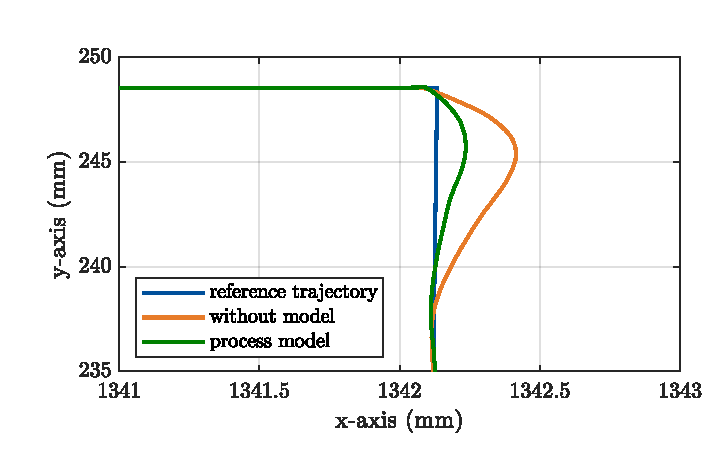
\includegraphics[width = 7.5cm]{Chapters/Experimental_Results/Experimental_Validation/EE_square.pdf}
   \vspace{-0.5cm}
  \caption{Reference and actual trajectory of the end-effector in Cartesian space.}
  \label{fig:ExpValProcess2}
  \vspace{-0.2cm}
\end{figure}

In general both process-based models perform similar to the models A and B which were derived from a classical parameter identification. This shows that the process based-models are suitable for practical application.% On average the model based feed-forward control scheme, utilizing the process models, reduces the control error by a factor of 3. This shows that the process based models are suitable for practical application.
% !TEX encoding = UTF-8 Unicode
% !TEX spellcheck = en_US
% !TEX root = ../../ICMA2020.tex

\section{Conclusion}
\label{sec:Conclusion}

When a robot is installed in its industrial environment the working area is highly restricted and parameter identification of robot's inverse dynamic models is a challenge. Satisfactory parameter identifiability can still be expected from optimized trajectories, but the optimization procedure is time-consuming and difficult to integrate into the software of the industrial controller. Therefore, in this paper identification during the final operation of the robot with in-process trajectories is investigated, which eliminates the need for dedicated identification experiments. 
Identifiability of the model parameters is now ensured by optimizing the composition of the model rather than the trajectory. A reduced-order model results including only those parameters that are relevant for the given in-process trajectory and parameter drift due to insufficient excitation is avoided.

In validation experiments with a serial robot it is shown that even with optimal excitation not all parameters can be identified if the workspace is restricted. For a simple in process trajectory only a few model parameters are relevant and accordingly the reduced order model is clearly simpler but approximately equally good.

The procedure is easy to use and requires no prior knowledge on the parameters. It can readily be integrated into the process control and requires no preparatory experiments. This makes it suitable for an industrial context.
% !TEX encoding = UTF-8 Unicode
% !TEX spellcheck = en_US
% !TEX root = ../../ICMA2020.tex

\section*{Acknowledgment and Remark}


We wish to thank Jonas Diekmeyer for creating the robot model.
%
\textsc{Matlab} code to reproduce the results is available at  
%
github.com/SchapplM/robotics-paper\_icma2020.
%\url{github.com/SchapplM/robotics-paper_icma2020}.

%https://github.com/SchapplM/robotics-paper_icma2020

% !TEX encoding = UTF-8 Unicode
% !TEX spellcheck = en_US

% !TEX encoding = UTF-8 Unicode
% !TEX spellcheck = en_US

\appendices
\label{sec:Appendix}
\section{Minimal Dynamics Parameter Vector}
\label{sec:MinparamVector}

The used Parameters are the mass $m_j$, the center of mass $\boldsymbol{r}_j$ in the coordinate system $(KS)_j$, the inertia $_{(j)}\boldsymbol{J}_j^{(j)}$ in the coordinate system $(KS)_j$, the motor and gear inertia $J_{Aj}$ as well as the Coulomb and viscous friction $f_{cj}$ and $f_{vj}$ for the joints $j=1,\ldots,6$ respectively. 
The combined masses $m_{123456}$, $m_{23456}$, $m_{3456}$ and $m_{456}$ are defined in \eqref{eq:MassenSumme}. The notation for $\boldsymbol{r}_j$ and $_{(j)}J_j^{(j)}$ is given in \eqref{eq:Komponentenschreibweise}.

\begin{equation}
\label{eq:Komponentenschreibweise}
	\boldsymbol{r}_j = 
		\begin{pmatrix}
		r_{jx} \\
		r_{jy} \\
		r_{jz} \\
		\end{pmatrix}
	\text{ ; }
	_{(j)}\boldsymbol{J}_j^{(j)} = 
		\begin{pmatrix}
		J_{jxx} & J_{jxy} & J_{jxz} \\
		J_{jxy} & J_{jyy} & J_{jyz} \\
		J_{jxz} & J_{jyz} & J_{jzz} \\
		\end{pmatrix}
\end{equation}


{\footnotesize
\begin{equation}
\label{eq:Parametersatz}
	\boldsymbol{\theta} = 
		\begin{pmatrix}
			J_{1yy} + 2 l_2 m_1 r_{1x} + l_2^2 m_{123456} + J_{A1} + J_{2yy} - l_3^2 m_{23456} + J_{3zz} - l_4^2 m_{3456} \\
			l_3^2 m_{23456} + J_{2xx} - J_{2yy} \\
			- l_3 m_2 r_{2z} + l_3 m_3 r_{3y} + J_{2xy} \\
			- l_3^2 m_{23456} + J_{2zz} + J_{A2} \\
			l_3 m_{23456} + m_2 r_{2x} \\
			J_{3xx} -J_{3zz} + l_4^2 m_3 + J_{4zz} + 2 l_5 m_4 r_{4y} + (l_4^2 +l_5^2) m_{456} \\
			-l_4 m_3 r_{3y} + J_{3xy} \\
			J_{3xz} \\
			J_{3yy} - l_4^2 m_{3456} + J_{4zz} + 2l_5 m_4 r_{4y} + l_5^2 m_{456} \\
			J_{3yz} \\
			l_4 m_{3456} + m_3 r_{3x} \\
			l_5 m_{456} + m_3 r_{3z} + m_4 r_{4y} \\
			J_{A3} \\
			J_{4xx} - J_{4zz} + J_{5zz} \\
			J_{4yy} + J_{5zz} \\
			J_{A4} \\
			l_6^2 m_6 + 2 l_6 m_6 r_{6z} + J_{5xx} - J_{5zz} + J_{6yy} \\
			l_6^2 m_6 + 2 l_6 m_6 r_{6z} + J_{5yy} + J_{6yy} \\
			l_6 m_6 + m_5 r_{5z} + m_6 r_{6z} \\
			J_{A5} \\
			J_{6xx} - J_{6yy} \\
			J_{6zz} \\
			J_{A6} \\
			
			f_{c1} \\
			\vdots \\
			f_{c6} \\
			
			f_{v1} \\
            \vdots \\
			f_{v6} \\
		\end{pmatrix}
\end{equation}
}

%\begin{equation}
%\label{eq:MassenSumme}
%    \begin{aligned}
%	m_{123456} &= m_1 + m_2 + m_3 + m_4 + m_5 + m_6 \text{ ,}\\
%	m_{23456} &= m_2 + m_3 + m_4 + m_5 + m_6 \text{ ,} \\
%	m_{3456} &= m_3 + m_4 + m_5 + m_6 \text{ ,} \\
%	m_{456} &= m_4 + m_5 + m_6 \\
%    \end{aligned}
%\end{equation}

\begin{equation}
\label{eq:MassenSumme}
    m_{j..6}=\sum_{i=j}^{6} m_i
\end{equation}

\bibliographystyle{IEEEtran}
%\bibliographystyle{acm}
\bibliography{Literatur}

\end{document}


